\documentclass[twoside]{book}

% Packages required by doxygen
\usepackage{calc}
\usepackage{doxygen}
\usepackage{graphicx}
\usepackage[utf8]{inputenc}
\usepackage{makeidx}
\usepackage{multicol}
\usepackage{multirow}
\usepackage{textcomp}
\usepackage[table]{xcolor}

% Font selection
\usepackage[T1]{fontenc}
\usepackage{mathptmx}
\usepackage[scaled=.90]{helvet}
\usepackage{courier}
\usepackage{amssymb}
\usepackage{sectsty}
\renewcommand{\familydefault}{\sfdefault}
\allsectionsfont{%
  \fontseries{bc}\selectfont%
  \color{darkgray}%
}
\renewcommand{\DoxyLabelFont}{%
  \fontseries{bc}\selectfont%
  \color{darkgray}%
}

% Page & text layout
\usepackage{geometry}
\geometry{%
  a4paper,%
  top=2.5cm,%
  bottom=2.5cm,%
  left=2.5cm,%
  right=2.5cm%
}
\tolerance=750
\hfuzz=15pt
\hbadness=750
\setlength{\emergencystretch}{15pt}
\setlength{\parindent}{0cm}
\setlength{\parskip}{0.2cm}
\makeatletter
\renewcommand{\paragraph}{%
  \@startsection{paragraph}{4}{0ex}{-1.0ex}{1.0ex}{%
    \normalfont\normalsize\bfseries\SS@parafont%
  }%
}
\renewcommand{\subparagraph}{%
  \@startsection{subparagraph}{5}{0ex}{-1.0ex}{1.0ex}{%
    \normalfont\normalsize\bfseries\SS@subparafont%
  }%
}
\makeatother

% Headers & footers
\usepackage{fancyhdr}
\pagestyle{fancyplain}
\fancyhead[LE]{\fancyplain{}{\bfseries\thepage}}
\fancyhead[CE]{\fancyplain{}{}}
\fancyhead[RE]{\fancyplain{}{\bfseries\leftmark}}
\fancyhead[LO]{\fancyplain{}{\bfseries\rightmark}}
\fancyhead[CO]{\fancyplain{}{}}
\fancyhead[RO]{\fancyplain{}{\bfseries\thepage}}
\fancyfoot[LE]{\fancyplain{}{}}
\fancyfoot[CE]{\fancyplain{}{}}
\fancyfoot[RE]{\fancyplain{}{\bfseries\scriptsize Generated on Thu Apr 23 2015 12\-:47\-:33 for My Project by Doxygen }}
\fancyfoot[LO]{\fancyplain{}{\bfseries\scriptsize Generated on Thu Apr 23 2015 12\-:47\-:33 for My Project by Doxygen }}
\fancyfoot[CO]{\fancyplain{}{}}
\fancyfoot[RO]{\fancyplain{}{}}
\renewcommand{\footrulewidth}{0.4pt}
\renewcommand{\chaptermark}[1]{%
  \markboth{#1}{}%
}
\renewcommand{\sectionmark}[1]{%
  \markright{\thesection\ #1}%
}

% Indices & bibliography
\usepackage{natbib}
\usepackage[titles]{tocloft}
\setcounter{tocdepth}{3}
\setcounter{secnumdepth}{5}
\makeindex

% Hyperlinks (required, but should be loaded last)
\usepackage{ifpdf}
\ifpdf
  \usepackage[pdftex,pagebackref=true]{hyperref}
\else
  \usepackage[ps2pdf,pagebackref=true]{hyperref}
\fi
\hypersetup{%
  colorlinks=true,%
  linkcolor=blue,%
  citecolor=blue,%
  unicode%
}

% Custom commands
\newcommand{\clearemptydoublepage}{%
  \newpage{\pagestyle{empty}\cleardoublepage}%
}


%===== C O N T E N T S =====

\begin{document}

% Titlepage & ToC
\hypersetup{pageanchor=false}
\pagenumbering{roman}
\begin{titlepage}
\vspace*{7cm}
\begin{center}%
{\Large My Project }\\
\vspace*{1cm}
{\large Generated by Doxygen 1.8.6}\\
\vspace*{0.5cm}
{\small Thu Apr 23 2015 12:47:33}\\
\end{center}
\end{titlepage}
\clearemptydoublepage
\tableofcontents
\clearemptydoublepage
\pagenumbering{arabic}
\hypersetup{pageanchor=true}

%--- Begin generated contents ---
\chapter{Namespace Index}
\section{Namespace List}
Here is a list of all documented namespaces with brief descriptions\-:\begin{DoxyCompactList}
\item\contentsline{section}{\hyperlink{namespaceuserInfo}{user\-Info} }{\pageref{namespaceuserInfo}}{}
\end{DoxyCompactList}

\chapter{Hierarchical Index}
\section{Class Hierarchy}
This inheritance list is sorted roughly, but not completely, alphabetically\-:\begin{DoxyCompactList}
\item Test\-Case\begin{DoxyCompactList}
\item \contentsline{section}{test.\-Test\-String\-Methods}{\pageref{classtest_1_1TestStringMethods}}{}
\end{DoxyCompactList}
\item \contentsline{section}{user\-Info.\-user\-Info}{\pageref{classuserInfo_1_1userInfo}}{}
\end{DoxyCompactList}

\chapter{Class Index}
\section{Class List}
Here are the classes, structs, unions and interfaces with brief descriptions\-:\begin{DoxyCompactList}
\item\contentsline{section}{\hyperlink{classtest_1_1TestStringMethods}{test.\-Test\-String\-Methods} }{\pageref{classtest_1_1TestStringMethods}}{}
\item\contentsline{section}{\hyperlink{classuserInfo_1_1userInfo}{user\-Info.\-user\-Info} }{\pageref{classuserInfo_1_1userInfo}}{}
\end{DoxyCompactList}

\chapter{Namespace Documentation}
\hypertarget{namespaceuserInfo}{\section{user\-Info Namespace Reference}
\label{namespaceuserInfo}\index{user\-Info@{user\-Info}}
}
\subsection*{Classes}
\begin{DoxyCompactItemize}
\item 
class \hyperlink{classuserInfo_1_1userInfo}{user\-Info}
\end{DoxyCompactItemize}


\subsection{Detailed Description}
\begin{DoxyVerb}@package docstring\end{DoxyVerb}
 
\chapter{Class Documentation}
\hypertarget{classtest_1_1TestStringMethods}{\section{test.\-Test\-String\-Methods Class Reference}
\label{classtest_1_1TestStringMethods}\index{test.\-Test\-String\-Methods@{test.\-Test\-String\-Methods}}
}
Inheritance diagram for test.\-Test\-String\-Methods\-:\begin{figure}[H]
\begin{center}
\leavevmode
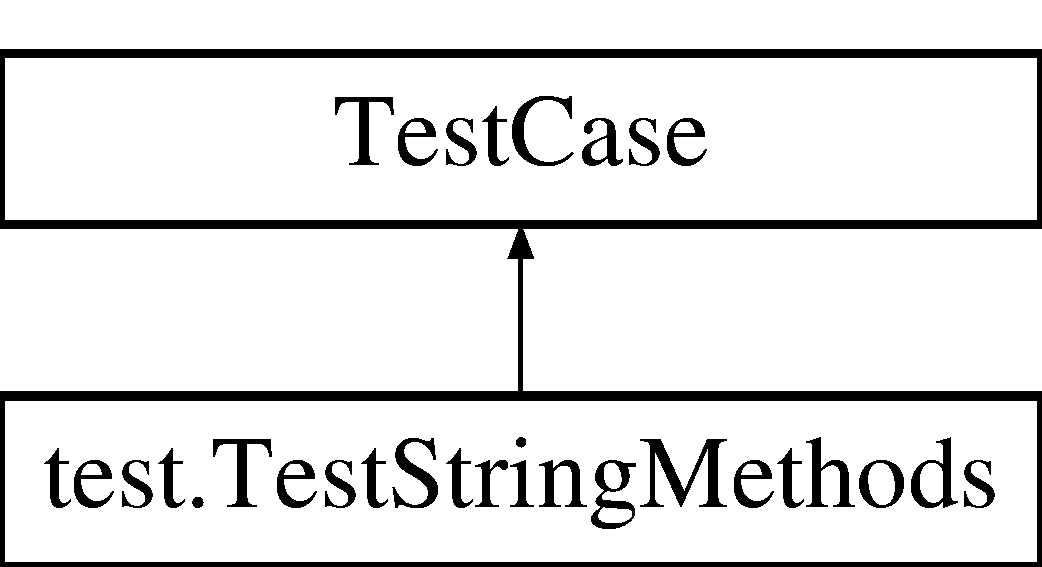
\includegraphics[height=2.000000cm]{classtest_1_1TestStringMethods}
\end{center}
\end{figure}
\subsection*{Public Member Functions}
\begin{DoxyCompactItemize}
\item 
def \hyperlink{classtest_1_1TestStringMethods_a1832baef4f040234656ffd378c2e6b81}{test\-\_\-in\-\_\-database}
\item 
def \hyperlink{classtest_1_1TestStringMethods_a81a9eaa19a51f16dbec286ac7731cb16}{test\-\_\-not\-\_\-in\-\_\-database}
\item 
def \hyperlink{classtest_1_1TestStringMethods_aa08b7eb60e48fd3579e3143bf1533c8a}{test\-\_\-upper\-\_\-lower\-\_\-mix}
\item 
def \hyperlink{classtest_1_1TestStringMethods_a840d5f836cbf6c2ff6921ad4b0b8fd86}{test\-\_\-one\-\_\-food\-\_\-calculation}
\item 
def \hyperlink{classtest_1_1TestStringMethods_a2f5e91a33f68511a76ae49d9797aa586}{test\-\_\-two\-\_\-food\-\_\-calculation}
\item 
def \hyperlink{classtest_1_1TestStringMethods_ad42efc3a8a28a05af1b62c49f766a6a2}{test\-\_\-three\-\_\-food\-\_\-but\-\_\-one\-\_\-not\-\_\-in\-\_\-database\-\_\-calculation}
\item 
def \hyperlink{classtest_1_1TestStringMethods_ae5e364e2ff8336f88eaeab28944b0715}{test\-\_\-none\-\_\-of\-\_\-food\-\_\-in\-\_\-database\-\_\-calculation}
\end{DoxyCompactItemize}


\subsection{Detailed Description}
\begin{DoxyVerb}This class uses to run the unit test for userInfo class
\end{DoxyVerb}
 

\subsection{Member Function Documentation}
\hypertarget{classtest_1_1TestStringMethods_a1832baef4f040234656ffd378c2e6b81}{\index{test\-::\-Test\-String\-Methods@{test\-::\-Test\-String\-Methods}!test\-\_\-in\-\_\-database@{test\-\_\-in\-\_\-database}}
\index{test\-\_\-in\-\_\-database@{test\-\_\-in\-\_\-database}!test::TestStringMethods@{test\-::\-Test\-String\-Methods}}
\subsubsection[{test\-\_\-in\-\_\-database}]{\setlength{\rightskip}{0pt plus 5cm}def test.\-Test\-String\-Methods.\-test\-\_\-in\-\_\-database (
\begin{DoxyParamCaption}
\item[{}]{self}
\end{DoxyParamCaption}
)}}\label{classtest_1_1TestStringMethods_a1832baef4f040234656ffd378c2e6b81}
\begin{DoxyVerb}This method uses to test if findFood function can find food in database
\end{DoxyVerb}
 \hypertarget{classtest_1_1TestStringMethods_ae5e364e2ff8336f88eaeab28944b0715}{\index{test\-::\-Test\-String\-Methods@{test\-::\-Test\-String\-Methods}!test\-\_\-none\-\_\-of\-\_\-food\-\_\-in\-\_\-database\-\_\-calculation@{test\-\_\-none\-\_\-of\-\_\-food\-\_\-in\-\_\-database\-\_\-calculation}}
\index{test\-\_\-none\-\_\-of\-\_\-food\-\_\-in\-\_\-database\-\_\-calculation@{test\-\_\-none\-\_\-of\-\_\-food\-\_\-in\-\_\-database\-\_\-calculation}!test::TestStringMethods@{test\-::\-Test\-String\-Methods}}
\subsubsection[{test\-\_\-none\-\_\-of\-\_\-food\-\_\-in\-\_\-database\-\_\-calculation}]{\setlength{\rightskip}{0pt plus 5cm}def test.\-Test\-String\-Methods.\-test\-\_\-none\-\_\-of\-\_\-food\-\_\-in\-\_\-database\-\_\-calculation (
\begin{DoxyParamCaption}
\item[{}]{self}
\end{DoxyParamCaption}
)}}\label{classtest_1_1TestStringMethods_ae5e364e2ff8336f88eaeab28944b0715}
\begin{DoxyVerb}This method uses to test if calculateCal function can return correct calories for all food are not in database
\end{DoxyVerb}
 \hypertarget{classtest_1_1TestStringMethods_a81a9eaa19a51f16dbec286ac7731cb16}{\index{test\-::\-Test\-String\-Methods@{test\-::\-Test\-String\-Methods}!test\-\_\-not\-\_\-in\-\_\-database@{test\-\_\-not\-\_\-in\-\_\-database}}
\index{test\-\_\-not\-\_\-in\-\_\-database@{test\-\_\-not\-\_\-in\-\_\-database}!test::TestStringMethods@{test\-::\-Test\-String\-Methods}}
\subsubsection[{test\-\_\-not\-\_\-in\-\_\-database}]{\setlength{\rightskip}{0pt plus 5cm}def test.\-Test\-String\-Methods.\-test\-\_\-not\-\_\-in\-\_\-database (
\begin{DoxyParamCaption}
\item[{}]{self}
\end{DoxyParamCaption}
)}}\label{classtest_1_1TestStringMethods_a81a9eaa19a51f16dbec286ac7731cb16}
\begin{DoxyVerb}This method uses to test if findFood function return false for food not in databases
\end{DoxyVerb}
 \hypertarget{classtest_1_1TestStringMethods_a840d5f836cbf6c2ff6921ad4b0b8fd86}{\index{test\-::\-Test\-String\-Methods@{test\-::\-Test\-String\-Methods}!test\-\_\-one\-\_\-food\-\_\-calculation@{test\-\_\-one\-\_\-food\-\_\-calculation}}
\index{test\-\_\-one\-\_\-food\-\_\-calculation@{test\-\_\-one\-\_\-food\-\_\-calculation}!test::TestStringMethods@{test\-::\-Test\-String\-Methods}}
\subsubsection[{test\-\_\-one\-\_\-food\-\_\-calculation}]{\setlength{\rightskip}{0pt plus 5cm}def test.\-Test\-String\-Methods.\-test\-\_\-one\-\_\-food\-\_\-calculation (
\begin{DoxyParamCaption}
\item[{}]{self}
\end{DoxyParamCaption}
)}}\label{classtest_1_1TestStringMethods_a840d5f836cbf6c2ff6921ad4b0b8fd86}
\begin{DoxyVerb}This method uses to test if calculateCal function can return correct calories for one food
\end{DoxyVerb}
 \hypertarget{classtest_1_1TestStringMethods_ad42efc3a8a28a05af1b62c49f766a6a2}{\index{test\-::\-Test\-String\-Methods@{test\-::\-Test\-String\-Methods}!test\-\_\-three\-\_\-food\-\_\-but\-\_\-one\-\_\-not\-\_\-in\-\_\-database\-\_\-calculation@{test\-\_\-three\-\_\-food\-\_\-but\-\_\-one\-\_\-not\-\_\-in\-\_\-database\-\_\-calculation}}
\index{test\-\_\-three\-\_\-food\-\_\-but\-\_\-one\-\_\-not\-\_\-in\-\_\-database\-\_\-calculation@{test\-\_\-three\-\_\-food\-\_\-but\-\_\-one\-\_\-not\-\_\-in\-\_\-database\-\_\-calculation}!test::TestStringMethods@{test\-::\-Test\-String\-Methods}}
\subsubsection[{test\-\_\-three\-\_\-food\-\_\-but\-\_\-one\-\_\-not\-\_\-in\-\_\-database\-\_\-calculation}]{\setlength{\rightskip}{0pt plus 5cm}def test.\-Test\-String\-Methods.\-test\-\_\-three\-\_\-food\-\_\-but\-\_\-one\-\_\-not\-\_\-in\-\_\-database\-\_\-calculation (
\begin{DoxyParamCaption}
\item[{}]{self}
\end{DoxyParamCaption}
)}}\label{classtest_1_1TestStringMethods_ad42efc3a8a28a05af1b62c49f766a6a2}
\begin{DoxyVerb}This method uses to test if calculateCal function can return correct calories for three food but not in database
\end{DoxyVerb}
 \hypertarget{classtest_1_1TestStringMethods_a2f5e91a33f68511a76ae49d9797aa586}{\index{test\-::\-Test\-String\-Methods@{test\-::\-Test\-String\-Methods}!test\-\_\-two\-\_\-food\-\_\-calculation@{test\-\_\-two\-\_\-food\-\_\-calculation}}
\index{test\-\_\-two\-\_\-food\-\_\-calculation@{test\-\_\-two\-\_\-food\-\_\-calculation}!test::TestStringMethods@{test\-::\-Test\-String\-Methods}}
\subsubsection[{test\-\_\-two\-\_\-food\-\_\-calculation}]{\setlength{\rightskip}{0pt plus 5cm}def test.\-Test\-String\-Methods.\-test\-\_\-two\-\_\-food\-\_\-calculation (
\begin{DoxyParamCaption}
\item[{}]{self}
\end{DoxyParamCaption}
)}}\label{classtest_1_1TestStringMethods_a2f5e91a33f68511a76ae49d9797aa586}
\begin{DoxyVerb}This method uses to test if calculateCal function can return correct calories for two food
\end{DoxyVerb}
 \hypertarget{classtest_1_1TestStringMethods_aa08b7eb60e48fd3579e3143bf1533c8a}{\index{test\-::\-Test\-String\-Methods@{test\-::\-Test\-String\-Methods}!test\-\_\-upper\-\_\-lower\-\_\-mix@{test\-\_\-upper\-\_\-lower\-\_\-mix}}
\index{test\-\_\-upper\-\_\-lower\-\_\-mix@{test\-\_\-upper\-\_\-lower\-\_\-mix}!test::TestStringMethods@{test\-::\-Test\-String\-Methods}}
\subsubsection[{test\-\_\-upper\-\_\-lower\-\_\-mix}]{\setlength{\rightskip}{0pt plus 5cm}def test.\-Test\-String\-Methods.\-test\-\_\-upper\-\_\-lower\-\_\-mix (
\begin{DoxyParamCaption}
\item[{}]{self}
\end{DoxyParamCaption}
)}}\label{classtest_1_1TestStringMethods_aa08b7eb60e48fd3579e3143bf1533c8a}
\begin{DoxyVerb}This method uses to test if findFood function can find food that are mixed string (lower and upper characters)
\end{DoxyVerb}
 

The documentation for this class was generated from the following file\-:\begin{DoxyCompactItemize}
\item 
test.\-py\end{DoxyCompactItemize}

\hypertarget{classuserInfo_1_1userInfo}{\section{user\-Info.\-user\-Info Class Reference}
\label{classuserInfo_1_1userInfo}\index{user\-Info.\-user\-Info@{user\-Info.\-user\-Info}}
}
\subsection*{Public Member Functions}
\begin{DoxyCompactItemize}
\item 
def \hyperlink{classuserInfo_1_1userInfo_ad49633d7bf7bd27625cce3d4686b5b37}{find\-Food}
\item 
def \hyperlink{classuserInfo_1_1userInfo_a1f41fd1097c4b3401f5571b26602e965}{calculate\-Cal}
\end{DoxyCompactItemize}
\subsection*{Static Public Attributes}
\begin{DoxyCompactItemize}
\item 
\hypertarget{classuserInfo_1_1userInfo_aac40b4174c0fba076ae17d06366d7794}{dictionary {\bfseries dictfood} = \{'chickendrumstick'\-:53.\-5,'egg'\-:1.\-44,'milk'\-:0.\-54\}}\label{classuserInfo_1_1userInfo_aac40b4174c0fba076ae17d06366d7794}

\item 
\hypertarget{classuserInfo_1_1userInfo_a87af9a3fe46b033310c86b7d47a7ca68}{int {\bfseries total} = 0}\label{classuserInfo_1_1userInfo_a87af9a3fe46b033310c86b7d47a7ca68}

\end{DoxyCompactItemize}


\subsection{Detailed Description}
\begin{DoxyVerb}This class uses to find food in our database or API
    and change users' information in databases
    @param dicfood It use to store information of food in case if we cannot use API
    @param total It use to store the total calories of user
\end{DoxyVerb}
 

\subsection{Member Function Documentation}
\hypertarget{classuserInfo_1_1userInfo_a1f41fd1097c4b3401f5571b26602e965}{\index{user\-Info\-::user\-Info@{user\-Info\-::user\-Info}!calculate\-Cal@{calculate\-Cal}}
\index{calculate\-Cal@{calculate\-Cal}!userInfo::userInfo@{user\-Info\-::user\-Info}}
\subsubsection[{calculate\-Cal}]{\setlength{\rightskip}{0pt plus 5cm}def user\-Info.\-user\-Info.\-calculate\-Cal (
\begin{DoxyParamCaption}
\item[{}]{self, }
\item[{}]{string}
\end{DoxyParamCaption}
)}}\label{classuserInfo_1_1userInfo_a1f41fd1097c4b3401f5571b26602e965}
\begin{DoxyVerb}This method uses to check if the food name in our database or not.
    @param string It is the string name of food from the users.
    @return total calories
\end{DoxyVerb}
 \hypertarget{classuserInfo_1_1userInfo_ad49633d7bf7bd27625cce3d4686b5b37}{\index{user\-Info\-::user\-Info@{user\-Info\-::user\-Info}!find\-Food@{find\-Food}}
\index{find\-Food@{find\-Food}!userInfo::userInfo@{user\-Info\-::user\-Info}}
\subsubsection[{find\-Food}]{\setlength{\rightskip}{0pt plus 5cm}def user\-Info.\-user\-Info.\-find\-Food (
\begin{DoxyParamCaption}
\item[{}]{self, }
\item[{}]{name}
\end{DoxyParamCaption}
)}}\label{classuserInfo_1_1userInfo_ad49633d7bf7bd27625cce3d4686b5b37}
\begin{DoxyVerb}This method uses to check if the food name in our database or not.
    @param name It is the name of the food from the users.
    @return true if food in databases, false othewise
\end{DoxyVerb}
 

The documentation for this class was generated from the following file\-:\begin{DoxyCompactItemize}
\item 
user\-Info.\-py\end{DoxyCompactItemize}

%--- End generated contents ---
\chapter{PHP Documentation}
\section{Documentation for PHP script here}

Your text goes here.

\subsection{This is a sub heading}

This might be a function?


% Index
\newpage
\phantomsection
\addcontentsline{toc}{chapter}{Index}
\printindex

\end{document}
